%%%%%%%% DLS 2026 internal supplementary material %%%%%%%%%%%%%%%%%%%%%%%%%%%
\documentclass[conference,letterpaper,10pt]{IEEEtran}

\usepackage{microtype}
\usepackage{graphicx}
\usepackage{booktabs}
\usepackage{amsmath}
\usepackage{array}
\usepackage{longtable}
\usepackage[hypertexnames=false,hyperfootnotes=false]{hyperref}

% Match the main manuscript's inter-column clearance.
\setlength{\columnsep}{0.20in}

\begin{document}

\title{Supplementary Material: Precision Accounting for KV and Recurrent-State Caches in Hybrid LLM Serving}
\author{%
\IEEEauthorblockN{Junxi Tan\IEEEauthorrefmark{1},
Yinhao Xiao\IEEEauthorrefmark{2}, and Wencheng Yang\IEEEauthorrefmark{3}}
\IEEEauthorblockA{\IEEEauthorrefmark{1}School of Big Data and Artificial
Intelligence; \IEEEauthorrefmark{2}GDUFE--UCM Joint Institute\\
\IEEEauthorrefmark{1}\IEEEauthorrefmark{2}Guangdong University of Finance
\& Economics, Guangzhou, China\\
\IEEEauthorrefmark{3}School of Science, Engineering and Digital Technologies,
University of Southern Queensland, Queensland, Australia\\
Emails: \IEEEauthorrefmark{1}2677510433@qq.com,
\IEEEauthorrefmark{2}20191081@gdufe.edu.cn,
\IEEEauthorrefmark{3}wencheng.yang@unisq.edu.au}}
\maketitle

\section{Byte-exact parameter derivation}
\label{app:bytes}

The attention term includes all GQA layers. At fp16, each attention layer
stores K and V tensors with 512 elements per token and 2 bytes per element,
for 2,048 bytes per layer and token. At int4, K and V each use 256 packed
payload bytes and 8 metadata bytes. Their combined cost is
$2\times(256+8)=528$ bytes per layer and token.

Each GDN layer contains convolution and temporal state. The convolution state
remains bf16 in both configurations and uses 36,864 bytes. The temporal state
uses 1,048,576 bytes at fp32 and 524,288 bytes at bf16. Consequently,
\begin{align}
G^{\mathrm{layer}}_{\mathrm{fp32}} &= 36{,}864+1{,}048{,}576
 = 1{,}085{,}440,\\
G^{\mathrm{layer}}_{\mathrm{bf16}} &= 36{,}864+524{,}288
 = 561{,}152.
\end{align}
The complete layer state falls by 48.30\%, not 50\%.

\begin{table}[t]
\centering
\small
\caption{\textbf{Architecture-derived continuous-model parameters.} All
values are bytes. No parameter is fitted to allocator token counts.}
\label{tab:parameters}
\setlength{\tabcolsep}{4pt}
\begin{tabular}{lrrrr}
\toprule
Model & $A_f$ & $A_q$ & $G_{fp32}$ & $G_{bf16}$\\
\midrule
2B & 12,288 & 3,168 & 19,537,920 & 10,100,736\\
9B & 16,384 & 4,224 & 26,050,560 & 13,467,648\\
\bottomrule
\end{tabular}
\end{table}

The 2B model has six GQA layers and 18 GDN layers; the 9B model has eight and
24, respectively. Multiplying the per-layer values gives the parameters in
Table~\ref{tab:parameters}. The representative padded recurrent pages are
1,089,792 bytes at fp32 and 566,016 bytes at bf16. Padding therefore adds
4,352 and 4,864 bytes, respectively. The continuous model uses unpadded
architecture bytes; the discrete allocator uses the padded layout.

\section{Discrete allocator reconstruction}
\label{app:discrete}

Let $K$ be the GPU-block count, $H$ the recurrent cache-group count, $B$ the
attention block size, and $L$ the requested context. The allocator-equivalent
slot count and allocator token capacity are
\begin{equation}
S_{\mathrm{alloc}}=\frac{K}{H+\lceil L/B\rceil},\qquad
T_{\mathrm{alloc}}=\lfloor L S_{\mathrm{alloc}}\rfloor.
\end{equation}

For 2B/int4/4K with fp32 state, $K=3287$, $H=3$, and $B=2064$.
The denominator is $3+\lceil4096/2064\rceil=5$. Thus
$S_{\mathrm{alloc}}=657.4$ and $T_{\mathrm{alloc}}=2{,}692{,}710$.
With bf16 state, $K=6330$ and $B=1072$. The denominator is seven,
$S_{\mathrm{alloc}}=904.286$, and
$T_{\mathrm{alloc}}=3{,}703{,}954$.

Fractional slots are an allocator normalization, not fractional scheduler
admissions. They also do not establish admission of the integer floor under
prefill, decode, or latency constraints.

\section{Full-matrix and temporal checks}
\label{app:matrix}

The formal matrix contained 112 allocator cells and 52 matched fp32/bf16 core
pairs. Every pair favored bf16 temporal state. The median capacity gain was
15.44\%, with a range of 3.32--93.28\%. The corrected continuous-model
residual had a 2.3795\% median absolute magnitude, a 2.7955\% mean absolute
magnitude, and a 13.2134\% maximum absolute magnitude. Signed residuals
spanned $-5.1604\%$ to $+13.2134\%$.

The temporal rerun repeated the frozen matrix. Because the allocator is
deterministic for a fixed build and configuration, this was a reproducibility
check rather than an independent statistical replicate. All cell directions
agreed, and the maximum token difference was 1.42\%.

\section{Dependence-aware GSM8K analysis}
\label{app:gsm8k}

Each dataset seed samples 200 GSM8K items without replacement. Samples overlap
across seeds, producing 1,800 seed-item draws but only 1,017 unique items.
Pairwise seed overlap ranges from 19 to 39, with median 30. The primary
estimand is the mean paired difference over the observed seed-item draws.

\begin{figure*}[t]
\centering
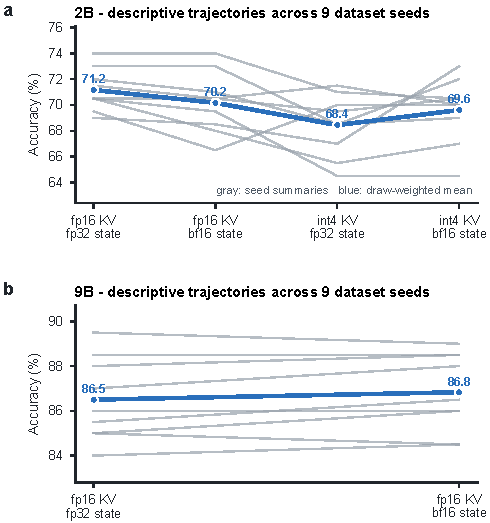
\includegraphics[width=0.72\textwidth]{figures/vector_redesign/fig8_gsm8k_per_seed.pdf}
\caption{\textbf{Descriptive GSM8K dataset-seed summaries.} Thin lines show
nine seed summaries. The blue line is the draw-weighted mean. These lines are
not independent replicates and are not the basis of the confidence intervals.}
\label{fig:seed-summaries}
\end{figure*}

For each candidate, an intercept-only OLS model is fit to paired binary
differences. The covariance uses two-way CR1 clustering by item and dataset
seed. The reference distribution is Student-$t$ with
$\min(1017-1,9-1)=8$ degrees of freedom. A percentile bootstrap samples the
1,017 item-level means with equal item weight for 20,000 replicates.

Repeated items were not always deterministic across dataset seeds despite
greedy decoding. The 2B full, state-only, KV-only, and joint allocations had
30, 27, 47, and 43 repeated items with inconsistent outcomes. Clustering
accounts for their dependence but does not explain the behavior. To prevent
reuse, the deprecated analysis that treated seed means as independent now
exits with an error.

\section{Additional evidence panels}
\label{app:figures}

\begin{figure*}[t]
\centering
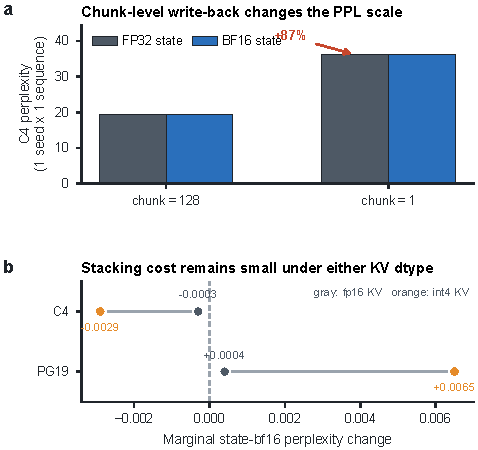
\includegraphics[width=0.72\textwidth]{figures/vector_redesign/fig7_harness.pdf}
\caption{\textbf{PPL harness boundary.} (a) Reducing chunk size from 128 to
one changes the PPL scale by about 87\%, so the harness is not equivalent to
per-token kernel semantics. (b) State contrasts under fp16 and int4 KV have
wide three-seed uncertainty and do not establish equivalence.}
\label{fig:harness}
\end{figure*}

\begin{figure*}[t]
\centering
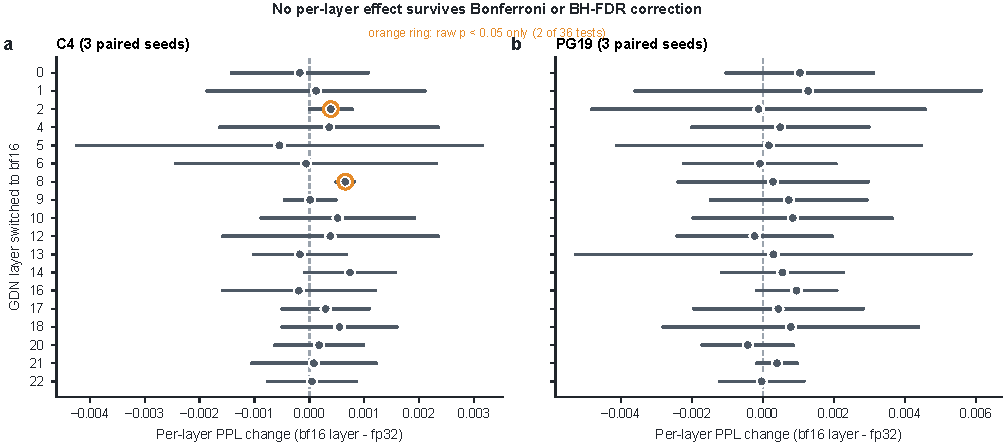
\includegraphics[width=\textwidth]{figures/vector_redesign/fig6_sensitivity.pdf}
\caption{\textbf{Exploratory per-layer sensitivity.} Two of 36 raw tests have
$p<0.05$. None survives Bonferroni or Benjamini--Hochberg correction. This
screen does not establish that whole-state precision is optimal.}
\label{fig:layers}
\end{figure*}

\section{Artifact and verification manifest}
\label{app:artifact}

The current submission does not claim a public artifact release. The
repository-local verifier checks SHA-256 digests for 16 frozen sources,
asserts headline values and all 52 paired capacity rows, and rejects obsolete
capacity inputs and GSM8K inputs based on seed-level independence. It also
checks all eight SVG/PDF pairs for nonempty vector output. Before producing
the JSON and LaTeX tables, the selector-audit generator verifies all four
decision sidecars.

\clearpage
\onecolumn
\section{Complete paired allocator matrix}
\label{app:full-matrix}

Table~\ref{tab:full-capacity} enumerates every fp32/bf16 pair in the formal
112-cell run. Model, KV data type, context length, and GPU-memory utilization
uniquely identify each pair. The remaining eight cells probe a float16-state
frontier and are not part of the 52-pair state comparison. The frozen source is
\texttt{capacity-phase-formal-corrected.analysis.json}; its SHA-256 prefix is
\texttt{879dc059579e}, with the full digest in the adjacent sidecar.

% Generated by scripts/bench/build_capacity_matrix_table.py.
% Source: results/verified/2026-08-14/capacity-phase-formal-corrected.analysis.json
% Source SHA-256: 879dc059579eff231b71d8c4513ee856a904e66791df84f8e8889da82173dd02
\begingroup
\scriptsize
\setlength{\tabcolsep}{3.0pt}
\renewcommand{\arraystretch}{0.94}
\setcounter{LTchunksize}{100}
\begin{longtable}{@{}llrrrrrrrr@{}}
\caption{\textbf{Complete formal allocator matrix.} $K$ is the allocated GPU-block count and $T$ is total allocator token capacity. Gain is $100(T_{16}/T_{32}-1)$; residual is the signed measured-to-continuous state-ratio error. The 52 rows come from attempt \texttt{capacity-phase-formal-20260811}; they are allocator measurements, not scheduler-admitted concurrency.}
\label{tab:full-capacity}\\
\toprule
Model & KV & $L$ & $u$ & $K_{32}$ & $K_{16}$ & $T_{32}$ & $T_{16}$ & Gain & Resid.\\
\midrule
\endfirsthead
\multicolumn{10}{l}{\tablename\ \thetable\ (continued)}\\
\toprule
Model & KV & $L$ & $u$ & $K_{32}$ & $K_{16}$ & $T_{32}$ & $T_{16}$ & Gain & Resid.\\
\midrule
\endhead
\midrule
\multicolumn{10}{r}{Continued on next page}\\
\endfoot
\bottomrule
\endlastfoot
2B & fp16 & 1,024 & 0.70 & 2,466 & 4,658 & 505,036 & 681,398 & 34.92\% & -4.72\% \\
2B & fp16 & 1,024 & 0.80 & 2,969 & 5,609 & 608,051 & 820,516 & 34.94\% & -4.70\% \\
2B & fp16 & 1,024 & 0.90 & 3,473 & 6,561 & 711,270 & 959,780 & 34.94\% & -4.71\% \\
2B & fp16 & 2,048 & 0.70 & 2,465 & 4,657 & 721,188 & 867,048 & 20.22\% & -5.16\% \\
2B & fp16 & 2,048 & 0.80 & 2,969 & 5,609 & 868,644 & 1,044,293 & 20.22\% & -5.16\% \\
2B & fp16 & 2,048 & 0.90 & 3,473 & 6,561 & 1,016,100 & 1,221,538 & 20.22\% & -5.16\% \\
2B & fp16 & 4,096 & 0.70 & 2,466 & 4,658 & 918,248 & 1,059,953 & 15.43\% & -0.16\% \\
2B & fp16 & 4,096 & 0.80 & 2,969 & 5,609 & 1,105,547 & 1,276,359 & 15.45\% & -0.14\% \\
2B & fp16 & 4,096 & 0.90 & 3,473 & 6,561 & 1,293,218 & 1,492,992 & 15.45\% & -0.15\% \\
2B & fp16 & 8,192 & 0.70 & 2,465 & 4,657 & 1,062,804 & 1,192,192 & 12.17\% & +3.37\% \\
2B & fp16 & 8,192 & 0.80 & 2,969 & 5,609 & 1,280,107 & 1,435,904 & 12.17\% & +3.36\% \\
2B & fp16 & 8,192 & 0.90 & 3,473 & 6,561 & 1,497,411 & 1,679,616 & 12.17\% & +3.36\% \\
2B & fp16 & 16,384 & 0.70 & 2,466 & 4,658 & 1,188,321 & 1,271,944 & 7.04\% & +2.46\% \\
2B & fp16 & 16,384 & 0.80 & 2,969 & 5,609 & 1,430,708 & 1,531,630 & 7.05\% & +2.48\% \\
2B & fp16 & 16,384 & 0.90 & 3,473 & 6,561 & 1,673,577 & 1,791,590 & 7.05\% & +2.48\% \\
2B & fp16 & 32,768 & 0.70 & 2,466 & 4,658 & 1,262,592 & 1,304,558 & 3.32\% & +1.01\% \\
2B & fp16 & 32,768 & 0.80 & 2,969 & 5,609 & 1,520,128 & 1,570,903 & 3.34\% & +1.03\% \\
2B & fp16 & 32,768 & 0.90 & 3,473 & 6,561 & 1,778,176 & 1,837,528 & 3.34\% & +1.03\% \\
2B & int4 & 1,024 & 0.70 & 2,515 & 4,843 & 643,840 & 1,239,808 & 92.56\% & +12.80\% \\
2B & int4 & 1,024 & 0.80 & 3,019 & 5,835 & 772,864 & 1,493,760 & 93.28\% & +13.21\% \\
2B & int4 & 1,024 & 0.90 & 3,545 & 6,826 & 907,520 & 1,747,456 & 92.55\% & +12.79\% \\
2B & int4 & 2,048 & 0.70 & 2,515 & 4,843 & 1,287,680 & 1,983,692 & 54.05\% & -1.81\% \\
2B & int4 & 2,048 & 0.80 & 3,030 & 5,835 & 1,551,360 & 2,390,016 & 54.06\% & -1.80\% \\
2B & int4 & 2,048 & 0.90 & 3,545 & 6,826 & 1,815,040 & 2,795,929 & 54.04\% & -1.81\% \\
2B & int4 & 4,096 & 0.70 & 2,515 & 4,843 & 2,060,288 & 2,833,846 & 37.55\% & -2.38\% \\
2B & int4 & 4,096 & 0.80 & 3,030 & 5,835 & 2,482,176 & 3,414,308 & 37.55\% & -2.37\% \\
2B & int4 & 4,096 & 0.90 & 3,545 & 6,826 & 2,904,064 & 3,994,185 & 37.54\% & -2.38\% \\
2B & int4 & 8,192 & 0.70 & 2,515 & 4,843 & 2,943,268 & 3,606,714 & 22.54\% & -2.88\% \\
2B & int4 & 8,192 & 0.80 & 3,030 & 5,835 & 3,545,965 & 4,345,483 & 22.55\% & -2.88\% \\
2B & int4 & 8,192 & 0.90 & 3,545 & 6,826 & 4,148,662 & 5,083,508 & 22.53\% & -2.89\% \\
2B & int4 & 16,384 & 0.70 & 2,515 & 4,822 & 3,745,978 & 4,158,086 & 11.00\% & -3.66\% \\
2B & int4 & 16,384 & 0.80 & 3,030 & 5,835 & 4,513,047 & 5,031,612 & 11.49\% & -3.24\% \\
2B & int4 & 16,384 & 0.90 & 3,545 & 6,805 & 5,280,116 & 5,868,058 & 11.14\% & -3.55\% \\
2B & int4 & 32,768 & 0.70 & 2,515 & 4,843 & 4,337,448 & 4,667,512 & 7.61\% & -0.62\% \\
2B & int4 & 32,768 & 0.80 & 3,030 & 5,835 & 5,225,633 & 5,623,567 & 7.62\% & -0.62\% \\
2B & int4 & 32,768 & 0.90 & 3,545 & 6,826 & 6,113,818 & 6,578,657 & 7.60\% & -0.63\% \\
9B & fp16 & 2,048 & 0.80 & 290 & 562 & 84,845 & 104,634 & 23.32\% & -2.71\% \\
9B & fp16 & 2,048 & 0.90 & 484 & 940 & 141,604 & 175,010 & 23.59\% & -2.50\% \\
9B & fp16 & 4,096 & 0.80 & 290 & 563 & 107,985 & 121,370 & 12.40\% & -2.79\% \\
9B & fp16 & 4,096 & 0.90 & 484 & 940 & 180,224 & 202,644 & 12.44\% & -2.75\% \\
9B & fp16 & 16,384 & 0.80 & 290 & 562 & 135,753 & 143,872 & 5.98\% & +1.45\% \\
9B & fp16 & 16,384 & 0.90 & 484 & 940 & 226,567 & 240,640 & 6.21\% & +1.67\% \\
9B & fp16 & 32,768 & 0.80 & 288 & 560 & 142,987 & 147,984 & 3.49\% & +1.18\% \\
9B & fp16 & 32,768 & 0.90 & 483 & 938 & 239,802 & 247,874 & 3.37\% & +1.06\% \\
9B & int4 & 2,048 & 0.80 & 287 & 567 & 146,944 & 232,243 & 58.05\% & +0.74\% \\
9B & int4 & 2,048 & 0.90 & 482 & 942 & 246,784 & 385,843 & 56.35\% & -0.34\% \\
9B & int4 & 4,096 & 0.80 & 288 & 559 & 235,929 & 327,094 & 38.64\% & -1.60\% \\
9B & int4 & 4,096 & 0.90 & 482 & 950 & 394,854 & 555,885 & 40.78\% & -0.08\% \\
9B & int4 & 16,384 & 0.80 & 288 & 567 & 428,962 & 488,933 & 13.98\% & -1.08\% \\
9B & int4 & 16,384 & 0.90 & 478 & 950 & 711,959 & 819,200 & 15.06\% & -0.14\% \\
9B & int4 & 32,768 & 0.80 & 286 & 564 & 493,244 & 528,032 & 7.05\% & -1.14\% \\
9B & int4 & 32,768 & 0.90 & 481 & 948 & 829,547 & 887,544 & 6.99\% & -1.19\% \\
\end{longtable}
\endgroup


\end{document}
